\chapter{肌肉结构和动力学} \label{chap:chap5}


如果你想理解功能,那就研究结构。

\begin{flushright}
	——弗朗西斯$\cdot$克里克
\end{flushright}


\begin{figure}[!htb]
	\centering
	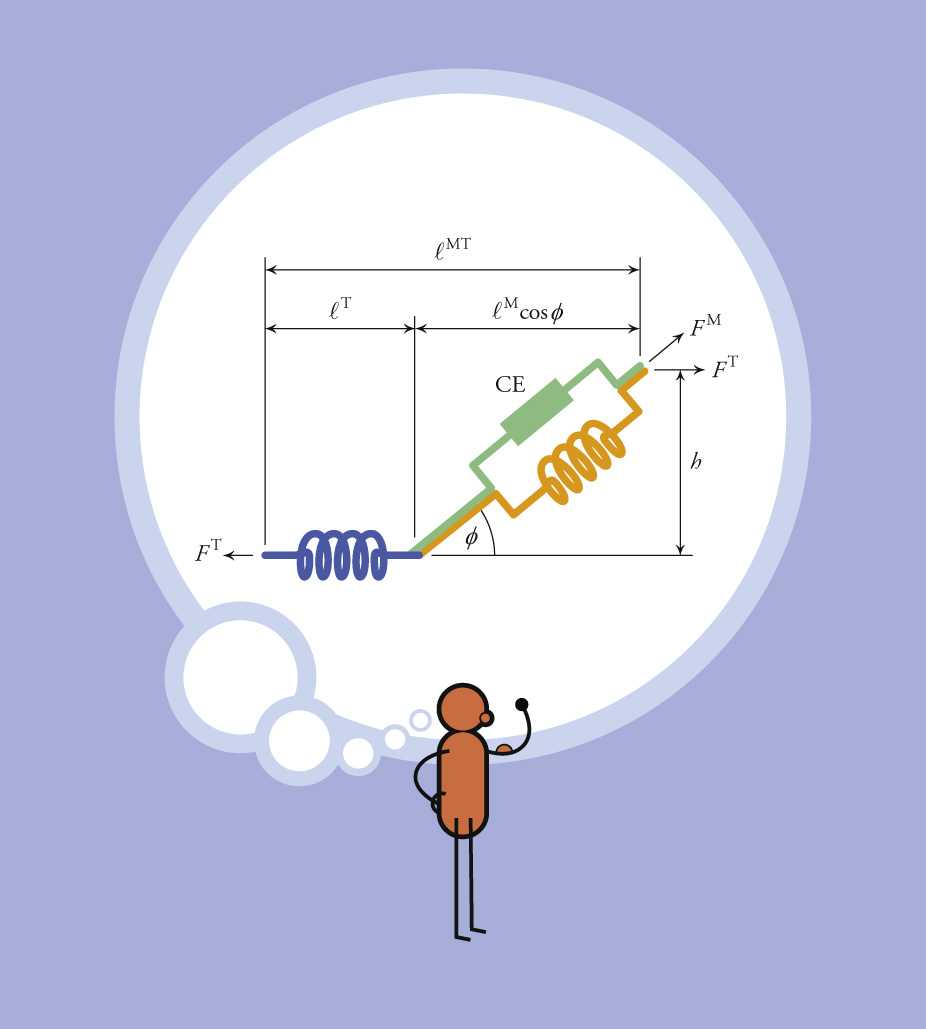
\includegraphics[width=1.0\linewidth]{chap5/5_0}
	% 加星号(*)表示不加编号
	\caption*{ \label{fig:5_0}}
\end{figure}


为了理解人类和动物的运动,研究人员开展了各种各样的实验。
生物力学家通过测量数千人的关节运动、地面反作用力和肌电信号来研究全身运动。
生理学家研究了单个肌肉,以表征肌肉激活和力量产生的动态。
肌肉驱动模拟使我们能够将这 2 个领域联系起来,将全身运动的生物力学测量与针对单个肌肉进行的实验相结合。
我们将在第~\ref{chap:chap10}~至~\ref{chap:chap12}~章中看到,肌肉驱动模拟可以深入了解肌肉在产生运动中的作用,并提供一些在人体运动时几乎无法测量的重要量估计值,例如肌肉产生的力量和它消耗的能量。


肌肉动力学建模对于创建肌肉驱动的运动模拟至关重要。
然而,一刀切的模型并不适用,因为每块肌肉都有其独特的结构来适应其独特的功能。
例如,一些肌肉负责手指的精细运动控制,而另一些肌肉则在运动过程中支撑身体重量(图~\ref{fig:5_1})。
所有骨骼肌都具有肌节的层级排列,但肌肉在几个重要方面存在差异。
这些差异包括它们的大小和结构,以及肌肉纤维的几何排列。
因此,肌肉的计算模型必须捕捉所有肌肉共同的肌肉力量产生特征,同时还要能够表征每块肌肉的独特特征。


\begin{figure}[!htb]
	\centering
	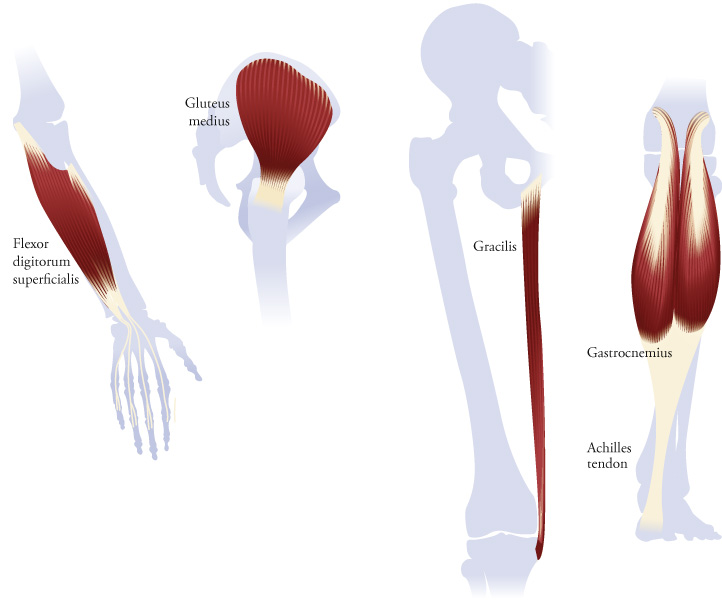
\includegraphics[width=1.0\linewidth]{chap5/5_1}
	\caption{全身肌肉的结构和功能各不相同。
		浅屈指肌(最左侧)通过 4 条肌腱控制手指屈曲;
		宽阔的臀中肌和纤细的股薄肌产生髋关节外展和内收力矩;
		腓肠肌(最右侧)通过较长的跟腱止于跟骨。 \label{fig:5_1}}
\end{figure}


在本章中,我们将了解如何创建一个通用的肌肉力量产生模型,以及如何对其进行定制以代表身体中的几乎任何肌肉。
我们将要描述的肌肉模型属于以 A. V. Hill 命名的一类模型,除了我们在第~\ref{chap:chap4}~章中看到的“推我拉你”实验之外,他还进行了许多肌肉的基础研究。
我的博士生导师 Felix Zajac 改进了 Hill 型模型,并将其带入了现代计算机模拟时代\cite{zajac1989muscle}。
具体来说,Zajac 开发了一个仅包含 4 条通用曲线和 5 个肌肉特定参数的模型,所有这些参数都可以从实验数据中得出并用于调整模型。
Zajac 模型的简单性对于涉及数十块肌肉的动态模拟至关重要,但它足够详细,可以表示不同大小、强度和结构的肌肉的动态。


图~\ref{fig:4_18}~总结了所有肌肉共同的肌肉力量产生特征。
这些特征包括 3 条曲线,描述肌肉长度与其产生的力之间的非线性关系:主动力-长度曲线、被动力-长度曲线和力-速度曲线。
由于肌肉通过肌腱附着在骨骼上,我们还必须考虑这种结缔组织的特性,我们用肌腱的力-长度曲线来描述它。
我们使用 5 个参数缩放这些通用曲线以表示特定的肌肉:
(1)最佳肌纤维长度 $l_o^M$;
(2)最佳纤维长度下的肌纤维羽状角 $\phi_o$ ;
(3)最大等长肌肉力量,$F_o^M$;
(4)最大肌肉收缩速度 $v_\text{max}^M$;
和(5)肌腱松弛长度,$l_s^T$。
本章首先介绍这 5 个特定于肌肉的参数。
我们将了解每个参数如何影响肌肉力量,并将其纳入肌肉-肌腱动力学模型中。


\section{最佳肌纤维长度$l_o^M$}

正如我们在第~\ref{chap:chap4}~章中看到的,肌节能够产生的主动力取决于其长度(图~\ref{fig:4_6})。
肌节能够产生最大等长收缩力的长度称为其最佳长度。
由于肌纤维由多个($n$)个首尾相连的肌节组成,因此肌纤维也存在一个最佳长度($l_o^M$),当其每个组成肌节都达到其最佳长度($l_o^S$)时,肌纤维便会达到该最佳长度:
%
\begin{equation}
	l_o^M = n l_o^S \label{eq:5_1}
\end{equation}

公式~\ref{eq:5_1}~假设肌纤维上串联的所有肌节长度相同。
肌肉在运动过程中会伸长和缩短,这会影响肌节粗肌丝和细肌丝相互滑动时产生的主动力。
最佳长度较长的肌纤维(即串联肌节较多)具有更宽的主动力-长度曲线,并且可以在更宽的长度范围内产生其最大主动力的很大一部分(图~\ref{fig:5_2}顶部)。
增加肌纤维的最佳长度也会增加其最大缩短速度():

\begin{figure}[!htb]
	\centering
	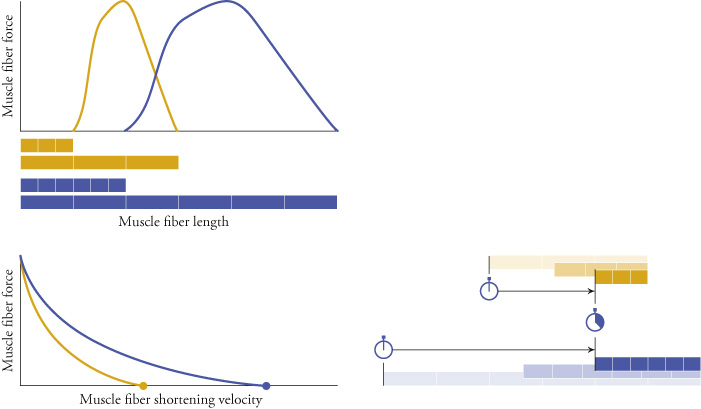
\includegraphics[width=1.0\linewidth]{chap5/5_2}
	\caption{最佳肌纤维长度较长的肌肉,其主动力-长度曲线(上图)更宽,最大缩短速度也更高(下图)。
		请注意,长肌纤维(蓝色)的示意图中,肌节数量是短肌纤维(橙色)的 2 倍,因此长肌纤维在给定时间内可以缩短 2 倍的距离(右下图)。 \label{fig:5_2}}
\end{figure}

\begin{equation}
	v_{\text{max}}^M = n v_{\text{max}}^S \label{eq:5_2}
\end{equation}
%
其中,$v_\text{max}^S$表示肌节的最大缩短速度。
因此,随着肌肉最佳纤维长度的增加,力-速度曲线也会变宽(图~\ref{fig:5_2}底部)。


生物肌肉由长度不同的肌束构成,肌束本身包含长度也不同的纤维,这些纤维甚至可能终止于肌束内。
然而,在我们的模型中,我们假设肌肉中的所有纤维长度相同(许多肌肉,但并非所有肌肉),肌腱动力学模型都做出了这一假设。
我们进一步假设所有纤维都是直的、平行的且共面的。
因此,为了表征肌肉的力-长度和力-速度特性,我们只是放大了肌纤维的相应特性,而这些特性仅仅是肌节相同特性的放大版本。



\section{最佳纤维长度下的肌纤维羽状角$\phi_o$}

肌肉通常通过肌腱附着于骨骼。
在平行纤维肌腱中(例如缝匠肌),其纤维沿着肌腱方向排列(图~\ref{fig:5_3})。
在大多数其他肌肉中,例如股直肌,其纤维与肌腱呈锐角排列;我们称这些肌肉为羽状肌。
“羽状肌”一词源于拉丁语,意为“羽毛状”,而羽状肌的结构确实让人联想到鸟类的羽毛。

\begin{figure}[!htb]
	\centering
	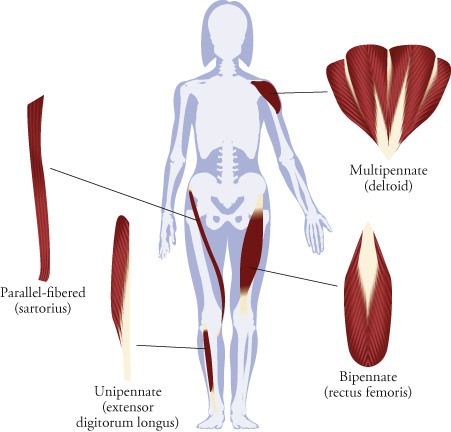
\includegraphics[width=0.8\linewidth]{chap5/5_3}
	\caption{具有不同结构肌肉的例子:
		平行纤维肌肉、单羽状肌肉、双羽状肌肉和多羽状肌肉。 \label{fig:5_3}}
\end{figure}

如果所有肌纤维都附着在肌腱的一侧,我们称该肌肉为单羽状肌;
如果肌纤维附着在肌腱的两侧,则称该肌肉为双羽状肌。
在多羽状肌中,肌腱分支和肌纤维结构可能很复杂。
因此,我们假设给定肌肉中的所有纤维都以相同的角度(称为羽状角 ($\phi$))附着于肌腱,并采用图~\ref{fig:5_4}~所示的肌肉-肌腱几何模型。
由此,我们得到肌纤维中的力 ($F^M$) 和肌腱中的力 ($F^T$) 之间的以下关系:

\begin{figure}[!htb]
	\centering
	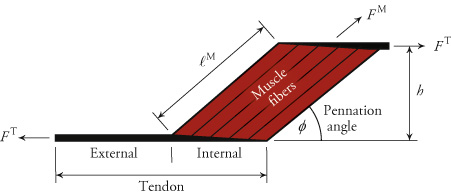
\includegraphics[width=0.75\linewidth]{chap5/5_4}
	\caption{肌纤维和肌腱的简化几何表示。
		肌纤维被假设为直的、平行的、共面的、等长的,并以相同的羽状角 ($\phi$) 附着于肌腱。
			当肌纤维缩短或伸长,羽状角增大或减小时,平行四边形的高度 $h$(以及面积)保持不变\cite{zajac1989muscle}。 \label{fig:5_4}}
\end{figure}

\begin{equation}
	F^T = F^M cos(\phi) 
	\label{eq:5_3}
\end{equation}

现在,参考图~\ref{fig:5_4},我们可以解释生物肌肉如何在纤维长度发生变化的情况下保持体积恒定。
随着图中纤维的缩短,想象一下它们以这样的方式缩短,使得图~\ref{fig:5_4}~中的平行四边形保持相同的高度 $h$。
平行四边形的顶部将保持不变,但底部将被向右拉,平行四边形将变得更接近矩形。
然而,只要高度保持不变,面积也将保持不变,这符合平行四边形面积等于其底边和高乘积的几何规则。
我们以二维方式绘制了该图,但三维运动类似,并确保肌肉的体积不变。
简而言之,羽状肌不是通过膨胀来维持体积,而是通过剪切来维持体积。


在上述过程中,羽状角不断增大,从纤维传递到肌腱的力不断减小,直到纤维与肌腱垂直,图中的肌肉呈矩形(即$\phi$ = 90度)。
我们使用参数$\phi_o$表示肌纤维达到最佳长度时的羽状角(即$l^M = l_o^M$)。
我们所描述的固定高度近似法可能会对收缩时明显隆起的肌肉引入误差,但它为研究肌肉结构的功能含义提供了一个简单的几何模型。


除了公式~\ref{eq:5_3}~中表达的关系外,羽状肌在决定肌肉的产力能力方面也起着至关重要的作用。
一般来说,羽状肌角度越大,在给定体积内能够容纳的肌肉纤维越多。
想象一下在矩形房间铺设硬木地板的类似情况:
可以使用相对较少的长木板来延伸房间的长度,或者使用大量较短的木板以对角线方向铺设。
同样,与相同体积的平行纤维肌肉相比,羽状肌的纤维更短,因此主动力-长度曲线和力-速度曲线更窄(图~\ref{fig:5_2})。
当然,羽状肌也包含更多的纤维,其后果将在下一节探讨。



\section{最大等长肌肉力 $F_o^M$}

我们 5 个肌肉参数系列中的第三个参数相对容易理解,但测量起来却不那么容易。
这就是最大等长肌肉力。
它被定义为肌肉在最大程度激活并保持最佳纤维长度时产生的力。


对于活体人体来说,最大等长肌力很难测量,因为我们无法将一块肌肉与其他肌肉分离,并只对该肌肉施加阻力。
因此,我们使用一个称为生理横截面积(PCSA;图~\ref{fig:5_5})的指标。
这是肌肉垂直于纤维方向的横截面积。
需要注意的是,在羽状肌中,该横截面积与肌肉的纵轴倾斜。
最大等长肌力可以通过以下方式估算:

\begin{figure}[!htb]
	\centering
	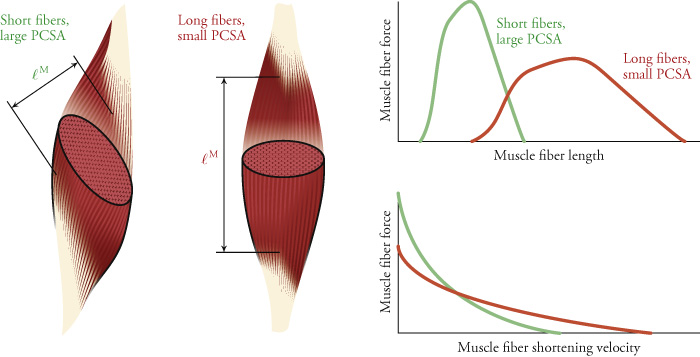
\includegraphics[width=1.0\linewidth]{chap5/5_5}
	\caption{左图所示的肌肉体积相同,但PCSA(主成分分析面积)、最佳纤维长度和羽状角不同。
		羽状肌越多,产生的主动力越大,但纤维越短;
		因此,其主动力-长度曲线和动力-速度曲线更高,但更窄\cite{lieber2002skeletal}。 \label{fig:5_5}}
\end{figure}

\begin{equation}
	F_o^M = \text{PCSA} \sigma_o^M
	\label{eq:5_4}
\end{equation}
%
其中 $\sigma_o^M$ 是肌肉的比张力(也称为峰值等长应力),即单位面积可产生的最大肌肉力。
在构建健康肌肉模型时,该参数的典型值为 $\sigma_o^M = 0.3 \; \text{MPa}$ 。


在上一节中,我们注意到,羽状肌的纤维比相同体积的平行纤维肌更短,但数量也更多。
因此,尽管羽状肌的力-长度和力-速度曲线较窄,但这些曲线也会更高,因为羽状肌的PCSA(以及因此产生的最大等长力)更大(图~\ref{fig:5_5})。


肌肉纤维的长度和收缩速度不仅仅受其几何形状的影响,我们将在接下来的两节中看到这一点。
尽管如此,我们已经可以观察到肌肉的结构如何影响其所能执行的功能范围:
在其他条件相同的情况下,羽状肌能够比相同体积的平行纤维肌产生更大的力量,但其长度范围较小,收缩速度也较低。



\section{最大肌肉收缩速度$v_\text{max}^M$}

到目前为止,我们已经介绍了 3 个与肌肉纤维几何排列相关的变量。
为了确定肌肉的最大收缩速度,我们现在引入一个概念:
肌肉纤维有 2 种类型:快肌纤维和慢肌纤维。
在单次收缩实验中(图~\ref{fig:4_12}),快肌纤维具有更快的上升时间和松弛时间,并且最大收缩速度也更高——大约为每秒 10 个最佳纤维长度 (10 $l_o^M / s$),而慢肌纤维约为 3 $l_o^M / s$ 个。
哺乳动物的肌肉同时包含这 2 种类型的纤维,但快肌纤维与慢肌纤维的比例会因肌肉的功能而异。
例如,腓肠肌含有大量的快肌纤维,这些纤维在需要快速产生巨大力量的活动(例如短跑)中被募集。
邻近的比目鱼肌主要由慢肌纤维组成,这些慢肌纤维非常适合在长时间站立时产生力量,因为慢肌纤维耐疲劳。


肌纤维不仅以其收缩速度区分,还以其产生ATP的方式区分。
有氧(即利用氧气)产生ATP的肌纤维比无氧(即无氧)产生ATP的肌纤维更耐疲劳。
慢肌纤维往往耐疲劳,而快肌纤维则易疲劳。
人类和其他一些动物拥有第三种肌纤维类型,因此我们通常将肌纤维分为I型(慢速,耐疲劳)、IIA型(快速,中度易疲劳)或IIB型(极快,高度易疲劳)。
通过强化训练可以增加快速且仅中度易疲劳的肌纤维比例。


回想一下第~\ref{chap:chap4}~章,运动单位大小各异,中枢神经系统会按照亨尼曼大小原则(图~\ref{fig:4_13})从小到大依次募集运动单位。
除了大小不同之外,运动单位所含纤维的类型也有所不同,同一运动单位中的所有纤维都属于同一类型。
最小的运动单位通常由 I 型纤维组成,最先被募集,其次是由 IIA 型纤维组成的稍大的运动单位。
最大的运动单位包含 IIB 型纤维,通常最后被募集。
因此,在低激活度下(例如在安静站立时可能观察到),主要募集的是慢肌、抗疲劳的运动单位。
因此,在低激活度下,肌肉的最大收缩速度可能会降低;
然而,在肌肉-肌腱动力学模型中,通常假设其为常数 10 $l_o^M/s$。


粗略地说,家禽和鱼类的可疲劳肌纤维和抗疲劳肌纤维是分开的(图~\ref{fig:5_6})。
相反,哺乳动物的肌肉中可疲劳肌纤维和抗疲劳肌纤维是交替分布的。
这就是为什么鸡肉菜肴可以用白肉或黑肉来制作,而牛肉菜肴却不能。
颜色差异的原因是深色肌肉(或肉)富含一种叫做肌红蛋白的蛋白质,这种蛋白质在肌肉中储存氧气,使肌肉颜色变深,使其更耐疲劳。
鸡腿的深色肉由用于长时间站立和奔跑的腿部肌肉(抗疲劳、慢肌纤维)组成。
白色的胸肉由仅用于短时间飞行的肌肉(可疲劳、快肌纤维)组成。
在人类中,单个肌纤维要么是“深色”的,要么是“白色”,但这两种纤维类型都散布在每块肌肉中。


\begin{figure}[!htb]
	\centering
	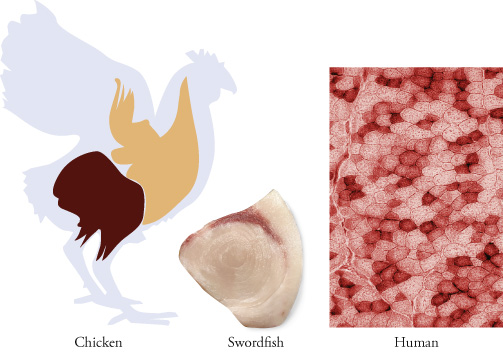
\includegraphics[width=0.8\linewidth]{chap5/5_6}
	\caption{鸡肉和鱼类的某些肌肉主要由抗疲劳的慢肌纤维(深色肉)组成,而另一些肌肉则由易疲劳的快肌纤维(白肉)组成。
		在人类和其他哺乳动物中,各种类型的纤维散布在每块肌肉中。
		人体纤维染色图像显示了不同的纤维类型,由 Richard Lieber 提供。 \label{fig:5_6}}
\end{figure}


\section{肌腱松弛长度 $l_s^T$}

到目前为止,我们讨论的所有参数都与肌腱无关。
在我们的希尔模型中,我们将肌腱描述为非线性弹簧。
本节介绍 5 个参数中的第五个参数,称为肌腱松弛长度,以及 4 个通用无量纲曲线中的第四个参数,称为肌腱力-长度曲线。
我们根据应力和应变之间的实验测量结果推导出力-长度曲线(图~\ref{fig:5_7})。


\begin{figure}[!htb]
	\centering
	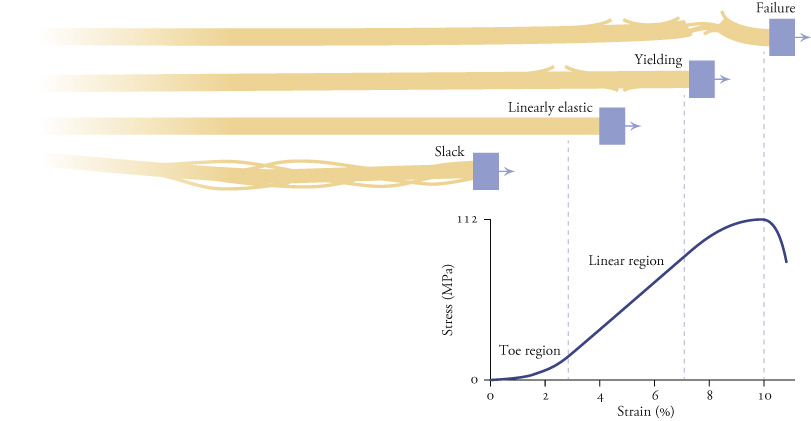
\includegraphics[width=0.8\linewidth]{chap5/5_7}
	\caption{在该图中,横轴表示肌腱的应变,用其长度相对于静止且未受力时的长度的百分比表示。
		静止长度即为松弛长度,用 $l_s^T$ 表示。
		任意给定时刻肌腱的应变 ($\epsilon^T$) 定义如下: \label{fig:5_7}}
\end{figure}

\begin{equation}
	\epsilon^T = \frac{l^T - l_s^T}{l_s^T} 
	\label{eq:5_5}
\end{equation}
% 
其中 $l^T$ 是肌腱的当前长度,$l_s^T$是其松弛长度。


图~\ref{fig:5_7}~中的纵轴表示肌腱单位横截面积产生的力,称为应力。
在线性弹簧中,应力与应变的关系图是一条直线,其斜率表示弹簧的刚度。
由于肌腱充当非线性弹簧,因此应力-应变曲线不是直线,并且它具有 3 个具有不同刚度特征的区域。
在脚趾区域,当肌腱拉伸约 0\% 到 3\% 时,它会更加柔顺(“有弹性”),随着肌腱的伸长和其组成胶原纤维的展开,其刚度逐渐增加。
在应力-应变曲线的线性区域,当肌腱拉伸约 3\% 到 7\% 时,肌腱具有恒定的刚度;
在此区域,它的行为类似于线性弹簧。
最后,超过 10\% 的应变,肌腱开始出现机械故障,并且存在很高的受伤风险。
我们通常假设内部肌腱(腱膜)和外部肌腱具有相同的材料特性和应变。
有实验证据支持上面给出的应变值,但有人认为肌腱在断裂前可以承受高达 15\% 的更高应变值。


肌腱会影响其所附着肌肉的长度,从而影响其产力能力(图~\ref{fig:5_8})。
如果肌腱的松弛长度相对于肌纤维的长度较短,则肌腱的拉伸几乎不会产生影响:
即使这样的肌腱承受很大的应变,其绝对长度变化(以及肌纤维缩短的量)也只是肌纤维最佳长度的一小部分。
相反,如果肌腱的松弛长度相对于肌纤维的最佳长度较长,则肌肉产力时肌腱会大幅拉伸,导致肌纤维明显缩短,并改变产生的主动力。
图~\ref{fig:5_9}~显示,较长的肌腱还可以增加肌肉-肌腱单元产力的长度范围。
通过这 2 种方式,肌腱都会显著影响肌肉功能。
当然,当肌腱损伤导致肌肉几乎无法使用时,肌腱的作用尤为明显。
正如我们将在第~\ref{chap:chap12}~章中看到的,肌腱在跑步过程中伸展和回缩时也在能量的储存和释放中发挥着重要作用。


\begin{figure}[!htb]
	\centering
	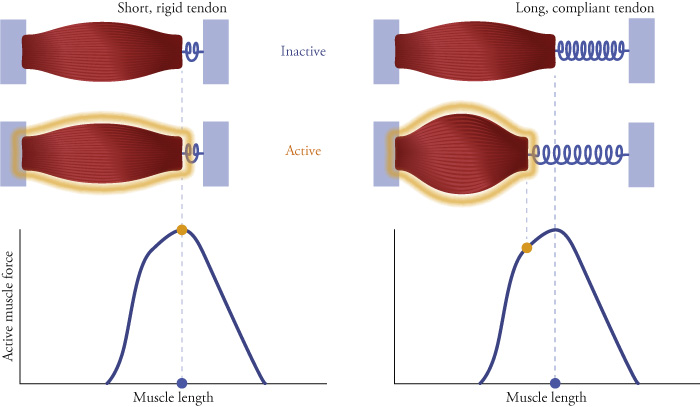
\includegraphics[width=1.0\linewidth]{chap5/5_8}
	\caption{肌腱的柔顺性会影响肌肉力量的产生。
		在图示的两种情况下,平行纤维肌肉在非活动状态时处于最佳长度(上)。
		如果肌腱相对较短且僵硬(左),则肌肉活动时肌纤维的长度变化可以忽略不计。
		如果肌腱较长且柔顺性良好(右),则肌肉活动时肌腱会拉伸,从而缩短肌纤维并减少产生的力量。 \label{fig:5_8}}
\end{figure}


\begin{figure}[!htb]
	\centering
	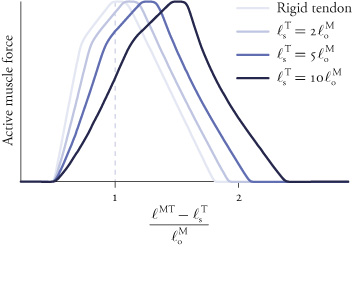
\includegraphics[width=0.6\linewidth]{chap5/5_9}
	\caption{肌腱柔顺性对主动力-长度曲线的影响。
		增加肌腱相对于最佳肌纤维长度的松弛长度(即增加肌腱柔顺性),可以扩大肌肉-肌腱执行器产生主动力的长度范围。 \label{fig:5_9}}
\end{figure}



\section{测量肌肉特定参数}

总而言之,我们定义了 5 个肌肉特异性参数,列于表~\ref{tab:5_1},这些参数捕捉了身体肌肉之间的大部分变异性。
我们在表 5.2 中列出了下肢主要肌肉的这些参数值。
为方便起见,我们通常将力、速度、肌肉长度和肌腱长度分别除以 、 、 和 来进行归一化,并使用波浪号表示归一化后的量(例如 )。


\begin{table}[htbp]
	\caption{Hill 型模型使用的 5 个肌肉特定参数} \label{tab:5_1} \centering
	\begin{tabular}{ccc} % l水平左居中,c水平居中
		\toprule
		肌肉特异性参数 & 符号 & 典型单位  \\
		\midrule
		最佳纤维长度下的羽状角 & $\phi_o$ &  度 \\
		\midrule
		最大等长力量 & $F_o^M$ &  牛顿 \\
		\midrule
		最大收缩速度 & $v_\text{max}^M$ &  $l_o^M / s$ \\
		\midrule
		肌腱松弛长度 & $l_s^T$ &  厘米 \\
		\bottomrule
	\end{tabular}
\end{table}


\begin{table}[htbp]
	\caption{下肢主要肌肉的肌肉特异性参数值*} \label{tab:5_2} \centering
	\begin{tabular}{ccccc} % l水平左居中,c水平居中
		\toprule
		肌肉 & 最大等长力(牛) & 最佳纤维长度(厘米)& 肌腱松弛长度(厘米) &  羽状角(度) \\
		\midrule
		短收肌 & 626 &  10.3 & 3.5 & 7 \\
		\midrule
		长收肌 & 917 &  10.8 & 13.2 & 8 \\
		\midrule
		大收肌 &  &   &  &  \\
		\midrule
		末梢 & 597 &  17.7 & 8.7 & 11 \\
		\midrule
		坐骨 & 597 &  15.6 & 21.6 & 10 \\
		\midrule
		腰部 & 597 &  13.8 & 4.7 & 12 \\
		\midrule
		近端 & 597 &  10.6 & 4.0 & 18 \\
		\midrule
		股二头肌长头 & 1313 &  9.8 & 32.5 & 10 \\
		\midrule
		股二头肌短头 & 557 &  11.0 & 10.6 & 15 \\
		\midrule
		伸趾长肌 & 603 &  6.9 & 36.9 & 13 \\
		\midrule
		拇长伸肌 & 286 &  7.5 & 32.7 & 11 \\
		\midrule
		屈趾长肌 & 423 &  4.5 & 37.9 & 13 \\
		\midrule
		拇长屈肌 & 908 &  5.3 & 35.4 & 15 \\
		\midrule
		腓肠肌外侧头 & 1575 &  5.9 & 37.6 & 12 \\
		\midrule
		腓肠肌内侧头 & 3116 &  5.1 & 39.9 & 10 \\
		\midrule
		臀大肌 &  &   &  &  \\
		\midrule
		上 & 984 &  14.7 & 4.9 & 20 \\
		\midrule
		中 & 1406 &  15.7 & 6.8 & 21 \\
		\midrule
		下 & 948 &  16.7 & 7.0 & 22 \\
		\midrule
		臀中肌 &  &   &  &  \\
		\midrule
		前 & 1093 &  7.3 & 5.6 & 18 \\
		\midrule
		中 & 765 &  7.3 & 6.5 & 18 \\
		\midrule
		后 & 871 &  7.3 & 4.5 & 18 \\
		%
		\midrule
		臀小肌 &  &   &  &  \\
		\midrule
		前 & 374 &  6.8 & 1.6 & 10 \\
		\midrule
		中 & 395 &  5.6 & 2.6 & 0 \\
		\midrule
		后 & 447 &  3.8 & 5.1 & 1 \\
		\midrule
		股薄肌 & 281 &  22.8 & 17.2 & 10 \\
		\midrule
		髂肌 & 1021 &  10.7 & 9.6 & 16 \\
		\midrule
		腓骨短肌 & 521 &  4.5 & 14.8 & 12 \\
		\midrule
		腓骨长肌 & 1115 &  5.1 & 33.2 & 14 \\
		\midrule
		梨状肌 & 1030 &  2.6 & 11.5 & 10 \\
		\midrule
		腰大肌 & 1427 &  11.7 & 10.0 & 12 \\
		\midrule
		股直肌 & 2192 &  7.6 & 44.9 & 12 \\
		\midrule
		缝匠肌 & 249 &  40.3 & 12.4 & 2 \\
		\midrule
		半膜肌 & 2201 &  6.9 & 34.8 & 15 \\
		\midrule
		半腱肌 & 591 &  19.3 & 24.7 & 14 \\
		\midrule
		比目鱼肌 & 6195 &  4.4 & 27.7 & 22 \\
		\midrule
		阔筋膜张肌 & 411 &  9.5 & 45.0 & 3 \\
		\midrule
		胫骨前肌 & 1227 &  6.8 & 24.1 & 11 \\
		\midrule
		胫骨后肌 & 1730 &  3.8 & 28.1 & 13 \\
		\midrule
		中间股 & 1697 &  9.9 & 20.2 & 4 \\
		\midrule
		股外侧肌 & 5149 &  9.9 & 22.1 & 15 \\
		\midrule
		股内侧肌 & 2748 &  9.7 & 20.0 & 24 \\
		\bottomrule
	\end{tabular}
\end{table}


目前已开发出多种技术来测量或计算肌肉和肌腱参数的值。
结构参数历来是通过对人类尸体进行测量获得的,而诸如力-速度关系的形状等动态特性通常来自动物肌肉实验。
获取和解释尸体测量值时必须小心谨慎,因为组织特性在死后可能会发生变化;
例如,肌肉脱水会改变肌肉的质量、体积、形状和长度。
此外,尸体测量数据通常取自老年捐赠者的遗体,他们的肌肉可能已经萎缩,因此无法代表经常参与研究的年轻健康受试者。
只要有可能,通常最好使用从被研究对象获得的测量值来校准肌肉骨骼模型,尤其是对于已知个体间差异很大的参数(例如最大等长力)。


肌纤维长度和羽状角可以通过解剖尸体标本或体内超声测量(图~\ref{fig:5_10},左)。
但请注意,最佳肌纤维长度无法通过超声图像确定,因为虽然可以测量肌纤维长度,但尚不清楚该长度与产生最大主动力的长度之间的关系。
肌节长度的测量提供了将测量的肌纤维长度与最佳肌纤维长度关联所需的信息,因为肌节的力-长度曲线是已知的。如果测量肌纤维长度 ($l^M$) 和肌节长度 ($l^S$),则最佳肌纤维长度 ($l_o^M$) 可按如下方式计算:


\begin{figure}[!htb]
	\centering
	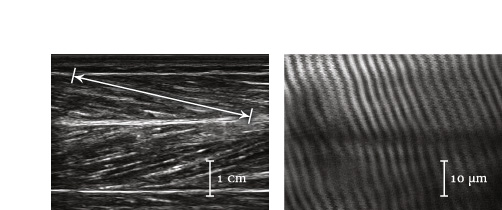
\includegraphics[width=0.75\linewidth]{chap5/5_10}
	\caption{成像技术提供了校准肌肉-肌腱动力学模型所需的数据。
		左图为胫骨前肌纤维的超声图像,可测量纤维长度。
		右图为使用双光子显微内窥镜获得的同一块肌肉的肌节图像,可测量肌节长度。
		图片由 Glen Lichtwark 和 Gabriel Sanchez 提供。 \label{fig:5_10}}
\end{figure}

\begin{equation}
	l_o^M = l^M \times \frac{l_o^S}{l^S}
	\label{eq:5_6}
\end{equation}
%
其中,表示肌节的最佳长度,人体肌肉中估计为 2.7 微米。
有几种技术可以测量整块肌肉的肌节长度。
其中一种方法是激光衍射法,该技术由 Richard Lieber 首创,通过手术暴露肌肉,然后用激光照射肌肉以产生衍射图案\cite{lieber1984sarcomere}。
我的实验室开发了一种侵入性较小的方法\cite{llewellyn2008minimally},使用针头大小的微型内窥镜对体内肌节长度进行成像(图~\ref{fig:5_10},右)。


由于腱膜位于肌肉内部,难以测量,因此在尸体标本或成像实验中难以确定肌腱松弛长度。
在肌肉-肌腱动力学模型中,确定肌腱松弛长度的一种策略是:测量尸体标本的肌纤维长度、肌节长度和关节位置,然后在模型中设定肌腱松弛长度,使肌纤维长度和肌节长度与同一姿势下的尸体测量值相匹配。


如前所述,我们可以通过测量PCSA和特定张力(公式~\ref{eq:5_4})来估算最大等长肌肉力量。
PCSA可以通过测量尸体标本的肌肉质量或使用MRI测量肌肉体积来估算,后者更可取,因为老年供体受试者的肌肉可能出现萎缩。
我们可以根据肌肉体积和最佳纤维长度计算PCSA,如下所示:
\begin{equation}
	\text{PCSA} = \frac{\text{muscle volume}}{l_o^M}
\end{equation}
%

在许多针对人体和动物肌肉的实验中,比张力的估算是通过计算最大测量肌肉张力与已知PCSA(纤维横截面积)的比值(参见公式~\ref{eq:5_4})来实现的。
请注意,文献中报告的PCSA值实际上可能是严格的几何横截面积,或者可能已经乘以了 $cos_(\phi)$。



\section{肌肉-肌腱动力学的希尔模型}

本节将基于 Hill\cite{hill1938heat}、Wilkie \cite{wilkie1956mechanical} 以及 Ritchie 和 Wilkie (1958) 的研究成果,描述一个广泛使用的肌肉-肌腱动力学模型。
A. V. Hill 在 20 世纪 30 年代进行了开创性的实验,以表征肌肉的力-速度特性。
此后,该模型得到了扩展,以捕捉我们之前描述的肌肉力产生过程中的其他显著特征。
尽管 Hill 只贡献了其中的一部分,但人们仍然习惯称之为“Hill 型模型”。


最流行的希尔型模型由三个部分组成:一个主动收缩元件和一个被动弹性元件,分别代表肌肉的主动和被动力产生特性;以及一个肌腱弹性元件(图~\ref{fig:5_11}A)。
这些元件的符号分别以绿色、橙色和蓝色表示,这些符号借鉴自工程文献。
我们将这三个元件的组合称为肌肉-肌腱执行器。
该模型用简单的元件来表示肌肉和肌腱;生物学的复杂性被提炼为定义这些元件动力学的参数和无量纲曲线。
当然,为了追求计算上易于处理的模型,我们省略了许多生物学细节。


\begin{figure}[!htb]
	\centering
	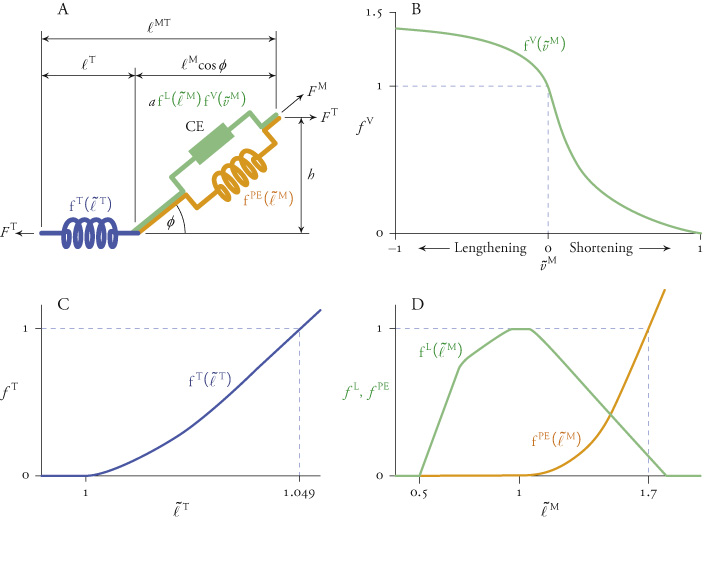
\includegraphics[width=0.75\linewidth]{chap5/5_11}
	\caption{典型的 Hill 型肌肉-肌腱模型示意图(A),以及描述其三个组成部分动力学的相应通用无量纲曲线:力-速度曲线(B)、肌腱力-长度曲线(C),以及主动和被动力-长度曲线(D)。
		图中所示的曲线来自 Millard 等人\cite{millard2013flexing},这些曲线是根据实验数据拟合的,与本文中显示的其他力-长度曲线有所不同。 \label{fig:5_11}}
\end{figure}


该模型常用于全身运动研究,因为它能够提供足够精确的肌肉力量估计,用于研究肌肉在行走和跑步过程中的动作,且计算量不大。
如前所述,肌腱弹性会显著影响肌肉纤维动力学,而肌肉与肌腱的相互作用是该模型的核心特征。
我们假设用一个非线性弹簧来表示肌腱对肌肉两端的影响,在力学上是等效的。
从图~\ref{fig:5_11}A~的示意图中可以看出,肌肉 ($l^M$)、肌腱 ($l^T$) 和肌肉-肌腱执行器 ($l^{MT}$) 的长度关系如下:
\begin{equation}
	l^{MT} = l^M cos(\phi) + l^T
	\label{eq:5_8}
\end{equation}



\section{无量纲曲线}

Hilltype 模型中三个组成部分的力生成特性可以用四条通用的、时不变的曲线来描述,列于表~\ref{tab:5_3},并如图~\ref{fig:5_11}B-D 所示。
一旦我们用肌肉特异性参数对这些曲线进行归一化,它们就变成了无量纲曲线。

\begin{table}[htbp]
	\caption{Hill 型模型使用的 4 条无量纲曲线} \label{tab:5_3} \centering
	\begin{tabular}{ccc} % l水平左居中,c水平居中
		\toprule
		\textbf{模型元素} & \textbf{无量纲曲线} & \textbf{符号}  \\
		\midrule
		主动收缩 & 主动力-长度 &  $f^L(\tilde{l} ^M)$ \\
		\midrule
		 & 力-速度 &  $f^V(\tilde{v} ^M)$ \\
		\midrule
		被动弹性 & 被动力-长度 &  $f^{PE}(\tilde{l} ^M)$ \\
		\midrule
		肌腱弹性 & 肌腱力-长度 &  $f^{T}(\tilde{l} ^T)$ \\
		\bottomrule
	\end{tabular}
\end{table}


通用曲线源自实验测量,反映了肌肉和肌腱的生物学特性。
具体而言,主动力-长度曲线是肌节长度与其激活时产生的力量之间关系的缩放版本(图~\ref{fig:4_6});
双曲线力-速度曲线反映了横桥骑行的动态(图~\ref{fig:4_9});
被动力-长度曲线表示肌肉在拉伸超过其静息长度时产生的力,与其激活无关(图~\ref{fig:4_7});
肌腱力-长度曲线表达了肌腱应变与其应力之间的非线性关系(图~\ref{fig:5_7})。
如图~\ref{fig:5_11}~中出现的归一化变量所示,四条通用的无量纲曲线通过肌腱的松弛长度($l_s^T$)和肌肉的最大等长力($F_o^M$)、最佳纤维长度($l_o^M$)和最大收缩速度($v_\text{max} ^M$)进行缩放。
肌腱力量与肌肉的最大等长力量成比例,因为一般来说,肌肉越强,肌腱就越强,从而避免肌腱衰竭。


缩放和使用无量纲曲线的重要性可以详细讨论,但重点在于,缩放使我们能够分离出模型中每个肌肉和个体独有的部分。
剩下的部分是所有健康肌肉共有的通用部分。



\section{利用刚性肌腱计算肌肉力量}

我们使用图~\ref{fig:5_11}~所示的希尔模型来生成肌肉驱动的运动模拟。
在本节中,我们将介绍构成图~\ref{fig:4_15}中“收缩动力学”模块的数学细节。
具体来说,我们将描述一种在已知肌肉激活度以及肌肉-肌腱执行器的长度和速度的情况下计算肌肉力的策略。
我们假设肌肉激活度已经由激活动力学模型计算出来,因此 $a(t)$ 是已知的。
我们还假设我们知道整个肌肉-肌腱执行器的长度和速度($l^{MT}(t)$ 和 $v^{MT}(t)$)。
但是,我们必须确定肌肉和肌腱的长度。
一旦知道这些长度,我们就可以使用肌肉特定参数以及图~\ref{fig:5_11}~所示的无量纲曲线来计算肌肉产生并通过肌腱传递的力
(请注意,为了简化符号,我们经常省略表示函数依赖时间的“($t$)”,但在本节和下一节中明确显示它,以区分时变量和常数。
还要注意,我们将肌纤维速度定义为缩短速度,以符合肌肉生理学文献和第~\ref{chap:chap4}~章中使用的惯例。
因此,在下面的等式中。)


让我们从一个更简单的问题开始,假设肌腱是刚性的;
然后在下一节中,我们将推广我们的策略,以解释弹性肌腱。
刚性肌腱假设将图~\ref{fig:5_11}A~所示的肌腱弹簧替换为刚性杆(即 $l^T$ 为常数)。
如果肌腱相对于其附着的肌肉较短,则该假设是合理的,在这种情况下,即使受到较大的拉力,肌腱也不会明显拉伸超过其松弛长度(回想一下图~\ref{fig:5_8})。
这样,我们在公式~\ref{eq:5_8}~中剩下 2 个未知数,并且可以将肌肉长度 ($l^M(t)$) 与肌纤维羽状角 ($\phi(t)$) 关联起来,如下所示:
%
\begin{equation}
	l^M(t) = \frac{
				l^{MT}(t) - l^T
			}{
				cos(\phi(t))
			}
	\label{eq:5_9}
\end{equation}

我们有一个方程,但有 2 个未知数。
为了取得进展,回想一下固定高度羽状模型,该模型将肌肉长度和羽状角与图~\ref{fig:5_4}~所示的平行四边形的高度 ($h$) 联系起来,该高度保持不变:
%
\begin{equation}
	h = l^M(t) sin(\phi(t))
	\label{eq:5_10}
\end{equation}

我们可以通过将最佳纤维长度 ($l_o^M$) 和最佳纤维长度处的羽状角 ($\phi_o$) 代入公式~\ref{eq:5_10}~来求解高度 $h$:
%
\begin{equation}
	h = l_o^M sin(\phi_o)
	\label{eq:5_11}
\end{equation}


现在,我们可以求解公式~\ref{eq:5_9}~和~\ref{eq:5_10},得到肌肉长度 ($l^M(t)$) 和羽状角 ($\phi(t)$),其中参数 $h$ 由公式~\ref{fig:5_11}~给出。
我们知道这个系统是可解的,因为独立方程的数量与未知数的数量相同。
将公式~\ref{fig:5_9}~代入公式~\ref{fig:5_10},可以得到羽状角的已知量表达式:
%
\begin{equation}
	\phi(t) = tan^{-1} (
				\frac{h}{
					l^{MT}(t) - l^T
				}
			)
	\label{eq:5_12}
\end{equation}
最后,我们可以使用公式~\ref{eq:5_9}~求解肌肉长度。


肌肉力量 ($F^M(t)$) 可以通过激活值 ($a(t)$)、标准化肌肉长度 ($\tilde{l}^M (t)$) 和标准化肌肉速度 ($\tilde{v} ^M (t)$) 来计算。
%
\begin{equation}
	F^M (t) = 
			F_o^M
			[
				a(t) f^L(\tilde{l}^M (t)) (\tilde{v}^M (t)) 
				+ f^{PE}(\tilde{l}^M (e))
			]
	\label{eq:5_13}
\end{equation}


这里我们将肌肉力的主动和被动分量相加,因为它们是并行作用的。
为了计算肌肉速度 ($v^M (t)$),我们注意到速度是长度的时间导数,并对公式~\ref{eq:5_8}~进行微分:
%
\begin{equation}
	v^{MT} (t) = - v^M(t) cos( \phi(t) )
				 - l^M(t) \dot{\phi}(t) sin( \phi (t) )
				 + v^T (t)
	\label{eq:5_14}
\end{equation}


回想一下,我们假设 $v^{MT}(t)$ 是已知的,而刚性腱假设告诉我们 $v^T(t) = 0$。
因此,公式~\ref{eq:5_14}~中只有 2 个未知数:
肌肉速度 ($v^M(t)$) 和羽状角速度 ($\dot{\phi} (t)$)。
2 个未知数,但只有一个方程。
幸运的是,我们也可以对公式~\ref{eq:5_10}~进行微分,得到与这 2 个变量相关的第二个方程:
%
\begin{equation}
	\hat{\phi (t)} = \frac{v^M (t)}{l^M (t)} tan(\phi (t))
	\label{eq:5_15}
\end{equation}


我们现在将公式~\ref{eq:5_15}~代入公式~\ref{eq:5_14}~来求解肌肉速度,最后使用公式~\ref{eq:5_13}~来计算肌肉力量。



\section{利用柔顺肌腱计算肌肉力量}

当肌腱是柔顺的而不是刚性的时,情况会更加复杂。
在这种情况下,肌腱的长度可以改变,因此 $l^T(t)$ 在公式~\ref{eq:5_9}~中是一个未知数。
处理这个额外未知数的一种策略是将肌肉长度 $l^M(t)$ 定义为状态变量,即在模拟过程中从一个时刻到下一个时刻进行数值积分的量。
该过程的工作原理如下。
我们提供时间零点的肌肉长度的初始值 ($l^M(t)$)、描述肌肉长度变化速率的方程(即其速度 vM(t))以及用于根据肌肉当前长度和速度计算未来短时间长度的数值积分器。
图~\ref{fig:4_15}~中的“收缩动力学”块将具有图~\ref{fig:5_12}~所示的形式。


\begin{figure}[!htb]
	\centering
	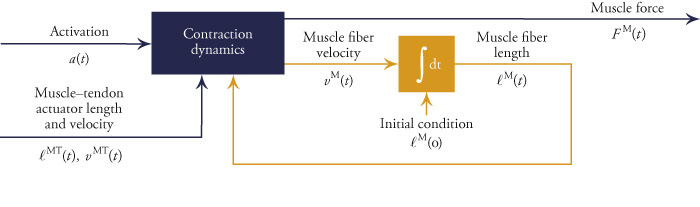
\includegraphics[width=1.0\linewidth]{chap5/5_12}
	\caption{肌纤维长度($l^M(t)$)随时间向前积分,以计算柔顺肌腱的收缩动力学。 \label{fig:5_12}}
\end{figure}


使用简单的数值积分器,我们可以按如下方式计算未来的肌肉长度:
%
\begin{equation}
	l^M (t + \delta t) = l^M (t) - \delta t v^M (t)
	\label{eq:5_16}
\end{equation}
%
其中 $\delta t$ 是每个时间步长推进到未来的时间量(回想一下 $\dot{l} ^M (t) = -v ^M (t)$ )。
通过反复重复此过程,我们最终获得了整个目标时间间隔内的肌肉长度值。使用公式~\ref{eq:5_16}~所示的积分策略(称为欧拉方法)通常需要我们采用较小的时间步长才能获得准确的答案。


现在,我们可以假设肌肉和肌腱无质量且无摩擦,从而推导出 $v^M(t)$ 的表达式,在这种情况下,它们相遇处没有净水平力。
因此,肌肉和肌腱处于平衡状态:
\begin{equation}
	F^T (t) = F^M (t) cos( \phi (t) )
	\label{eq:5_17}
\end{equation}

(因为在图~\ref{fig:5_11}A~中肌腱被限制为保持水平,所以我们可以忽略肌肉产生的力的垂直分量 $F^M(t) sin(\phi(t))$)。
肌腱产生的力 ($F^T(t)$) 可以根据标准化肌腱长度 ($\tilde{l} ^T (t)$) 使用肌腱力-长度曲线计算得出:
%
\begin{equation}
	F^T (t) = F_o ^M [
		f^T
		(
			\tilde{l} ^T (t)
		)
	]
	\label{eq:5_18}
\end{equation}

我们将肌肉和肌腱力的表达式(公式~\ref{eq:5_13}~和~\ref{eq:5_18})代入平衡方程(公式~\ref{eq:5_17})并求解,得到肌肉速度的表达式:
%
\begin{equation}
	\tilde{v} ^M (t) = 
		f_\text{inv} ^V
		(
			\frac{
				f^T (\tilde{l} ^T (T) / cos( \phi (t) ))
				- f^{PE} (\tilde{l} ^M (t))
			}{
				a(t) f^L ( \tilde{l}^M (t) )
			}
		)
	\label{eq:5_19}
\end{equation}
%
其中 $f_\text{inv} ^V$ 是力-速度曲线的倒数(即,它描述肌肉速度作为力的函数)。
请注意,公式~\ref{eq:5_19}~有 4 个数值奇异点,在模拟过程中必须避免:
当羽状角接近 90 度时、当激活度接近零时、当纤维长度达到主动力-长度曲线接近零时,以及当力-速度曲线不可逆时。
可以通过对相应变量引入约束来避免这些奇异点,例如,防止羽状角超过小于 90 度的某个上限。


上述方法用于估算几乎所有肌肉驱动运动模拟中的肌肉和肌腱力量。
该方法的价值在于,它使我们能够在估算每块肌肉产生的力量时,考虑其激活程度、纤维长度和纤维速度。
然而,其他方法也同样有用,我们将在下文中进行介绍。



\section{肌肉力量产生的其他模型}

我们重点关注希尔型模型,因为它广泛应用于运动模拟,包括本书介绍的运动模拟。
然而,希尔型模型未能捕捉到一些现象。
例如,该模型忽略了短程刚度(描述肌肉对长度小幅快速扰动产生的与速度无关的抵抗力);忽略了力量增强(即拉伸后肌肉最大等长收缩力的立即增加);以及对温度和疲劳的依赖性。
此外,虽然希尔型模型能够很好地表示肌肉在最大活动状态下,长度和速度变化引起的肌肉力量变化,但它对于次最大活动状态的准确性较低\cite{millard2013flexing}。
在科学研究中使用希尔型模型时,必须考虑这些局限性。


其他肌肉模型也已开发出来,有的更简单,有的更复杂。
一种简单的肌肉力建模策略是,用一个扭矩执行器(一种具有生理学特性的马达)来表示关节上所有肌肉产生的总力矩。
该执行器的最大扭矩可以表示为关节角度的函数,该角度由实验确定,但无法计算单个肌肉的力。
正如我们将看到的,该模型足够简单,可用于大规模优化问题,同时仍能产生与人类运动非常相似的模拟结果。


当需要更详细的信息来解答特定问题时,也有一些肌肉模型可以提供这些信息。
一个著名的例子是基于安德鲁$\cdot$赫胥黎\cite{huxley1957muscle}的研究,其中明确地模拟了肌肉收缩的滑动丝机制。
这个赫胥黎型模型使用以下形式的偏微分方程来描述力的产生:
%
\begin{equation}
	\frac{\partial n(x,t)}{\partial t}
	- v(t) \frac{\partial n(x,t)}{\partial x}
	= f(x)
	- ( f(x) + g(x) ) n(x,t)
	\label{eq:5_20}
\end{equation}
%
其中 $n(x,t)$ 是描述参与横桥循环的肌动蛋白和肌球蛋白比例的概率密度函数;
$x$ 和 $t$ 是距离和时间的独立变量;
$v(t)$ 是半肌节的缩短速度;
函数 $f(x)$ 和 $g(x)$ 分别表示横桥形成和断裂的速率。
使用该模型的主要挑战是确定模型中许多参数的适当值,因为我们对这些量在不同物种和不同肌肉之间的变化知之甚少。
尽管如此,该模型捕捉到了上述一些希尔型模型未能捕捉到的效应。
横桥模型通常用于研究单块肌肉的动力学。


有限元模型提供了另一种选择。
在有限元模型中,肌肉被划分为许多小单元(数量级达数千个),每个单元由一组描述组织行为的方程控制。
有限元模型是工程应用(例如飞机设计)的最新方法,毫无疑问,它们比我们在本章中推导的简单方程具有更高的精度。


但更强大的计算能力是有代价的:
有限元模型的求解时间比希尔型模型长数百倍。
尽管计算负担较大,有限元模型仍能有效地模拟纤维长度不一、应变不均匀且横向传递张力的肌肉(图~\ref{fig:5_13})。
最终,您必须在模型提供的细节量与其针对具体应用的分析可处理性之间找到适当的平衡。


\begin{figure}[!htb]
	\centering
	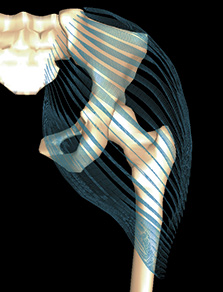
\includegraphics[width=0.4\linewidth]{chap5/5_13}
	\caption{Blemker\cite{blemker2005three}的臀大肌模型。
		有限元模型提供了肌肉结构的详细特征,并可以计算内部肌肉和肌腱的应变。 \label{fig:5_13}}
\end{figure}


由于许多肌肉参与运动的协调和控制,因此,对大量肌肉进行模拟对于研究步行和跑步等活动至关重要。
本章讨论的模型使我们能够仅使用少量计算资源一次模拟数十块肌肉。
我们将在第~\ref{chap:chap10}~至~\ref{chap:chap12}~章中展示我们的计算能力,以生成肌肉驱动的运动模拟。



